\newpage
\section{Implementacja}

W tym rozdziale przedstawimy implementację algorytmu wyszukiwania w drzewie binarnym (BST) w języku C++. Skupimy się na najważniejszych fragmentach kodu, które implementują główne operacje takie jak dodawanie, usuwanie elementów oraz wyświetlanie drzewa. Omówimy także powstałe wyniki działania aplikacji oraz wprowadzone optymalizacje.

\subsection{Struktura kodu}

Aplikacja składa się z kilku głównych modułów:

\begin{itemize}
	\item \textbf{App.cpp} – implementacja interfejsu użytkownika, obsługi menu oraz wywołania odpowiednich funkcji na drzewie.
	\item \textbf{BinarySearchTree.cpp} – implementacja głównych operacji na drzewie wyszukiwań binarnych, takich jak dodawanie, usuwanie i przeglądanie drzewa.
	\item \textbf{main.cpp} – punkt wejścia do aplikacji, który uruchamia główną logikę programu.
\end{itemize}

Poniżej przedstawiamy przykłady implementacji najważniejszych funkcji.

\subsection{Dodawanie elementów do drzewa}

Funkcja \texttt{addItem} (listing \OznaczKod{addItem}) umożliwia dodanie elementu do drzewa. Implementacja opiera się na rekursji – w zależności od wartości elementu, funkcja dodaje nowy węzeł do lewego lub prawego poddrzewa.

\lstinputlisting[caption=Funkcja addItem, label={lst:addItem}, language=C++]{kod/addItem.cpp}

\textbf{Opis:} Funkcja sprawdza, czy węzeł jest pusty (czyli czy osiągnęliśmy koniec drzewa lub poddrzewa), a następnie tworzy nowy węzeł o zadanej wartości. Następnie przekazuje go do odpowiedniego poddrzewa (lewego lub prawego), aby odpowiednio uporządkować drzewo.

\subsection{Usuwanie elementów z drzewa}

Usuwanie elementu z drzewa (listing \OznaczKod{removeItem}) jest bardziej skomplikowane, ponieważ musi zachować strukturalną spójność drzewa. Istnieją trzy przypadki:

\begin{enumerate}
	\item Węzeł do usunięcia nie ma potomków – w takim przypadku po prostu usuwamy węzeł.
	\item Węzeł do usunięcia ma jedno dziecko – wówczas zastępujemy węzeł jego dzieckiem.
	\item Węzeł do usunięcia ma dwóch potomków – w takim przypadku należy znaleźć najmniejszy węzeł w prawym poddrzewie lub największy w lewym poddrzewie, zastąpić nim usuwany węzeł, a następnie usunąć ten węzeł rekurencyjnie.
\end{enumerate}

\lstinputlisting[caption=Funkcja removeItem, label={lst:removeItem}, language=C++]{kod/removeItem.cpp}

\textbf{Opis:} Rekursywne usuwanie węzła odbywa się poprzez analizowanie, w którą stronę należy przejść – do lewego lub prawego poddrzewa. Gdy znajdziemy węzeł do usunięcia, odpowiednio go usuwamy lub zastępujemy.

\subsection{Wyświetlanie drzewa}

Aby umożliwić wizualizację struktury drzewa, zaimplementowaliśmy funkcję \texttt{display} (listing \OznaczKod{display}), która umożliwia wyświetlenie drzewa w różnych porządkach: preorder, inorder oraz postorder.

\lstinputlisting[caption=Funkcja display, label={lst:display}, language=C++]{kod/display.cpp}

\textbf{Opis:} Funkcja ta wykonuje odpowiednią metodę przeglądania drzewa, przekazując wybrany typ porządku przeglądania do odpowiedniej funkcji rekurencyjnej.

\subsection{Wyniki implementacji}

Po zaimplementowaniu głównych funkcji aplikacja została przetestowana na różnych zbiorach danych. Drzewo binarne skutecznie obsługiwało operacje dodawania, usuwania oraz wyświetlania w różnych porządkach. Aplikacja jest wydajna i działa w czasie proporcjonalnym do liczby elementów w drzewie.

\begin{figure}[ht]
	\centering
	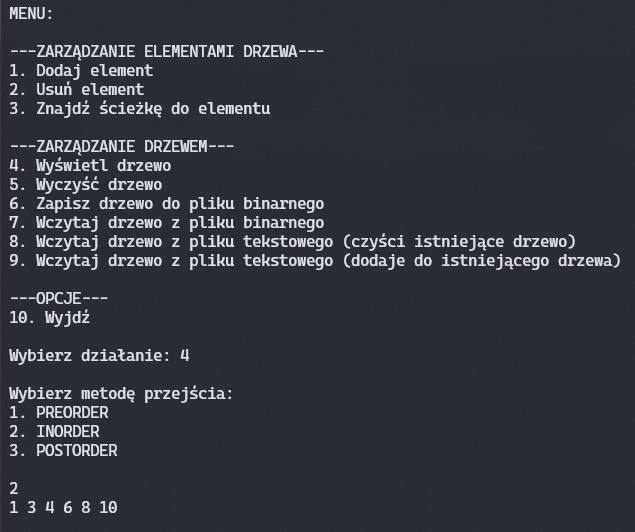
\includegraphics[width=0.7\textwidth]{rys/display_bst.png}
	\caption{Przykład wyników wyświetlania drzewa}
\end{figure}

\textbf{Wynik 1:} Wyświetlanie drzewa po kilku operacjach dodawania i usuwania elementów. Drzewo jest poprawnie zbalansowane i przedstawione w porządku inorder.
